\subsection{Level2.3: $y=-x*cos(x)$ について}
\subsubsection{プログラムソース(変更部分)}
\begin{breakbox}
\begin{verbatim}
行数 変更点
28 z = -x * cos(x);
36 z_dx = x * sin(x) - cos(x);
\end{verbatim}
\end{breakbox}

\begin{breakbox}
\begin{verbatim}
#!/bin/bash
set -e

# 図タイトル(func), シード値(seed) の取得。
if [ $# -eq 3 ] ; then
		seed1=$1
		seed2=$2
		seed3=$3
else
    echo "Usage: prompt> $0 \"gnuplot_style_func\" seed"
    exit 0
fi

# シミュレーション実行&データ抽出。
exec_file="./steepest_decent"
transition_file="./transition.txt"
exec_file1="./Compare"

if [ -f $transition_file ] ; then
    rm $transition_file
fi

for seed in $seed1 $seed2 $seed3
do
	archive_file=.archive-$seed
	$exec_file $seed > $archive_file
	cat $archive_file | cut -f2,4,6,8 -d" " > .data-$seed
done

echo "seed $seed1 finish f(x,y)" 
tail -c 14 .data-$seed1 | cut -c-13
seed1min=`tail -c 14 .data-$seed1 | cut -c-13 `

echo "seed $seed2 finish f(x,y)" 
tail -c 14 .data-$seed2 | cut -c-13
seed2min=`tail -c 14 .data-$seed2 | cut -c-13`

echo "seed $seed3 finish f(x,y)" 
tail -c 14 .data-$seed3 | cut -c-13
seed3min=`tail -c 14 .data-$seed3 | cut -c-13`


echo "最適解は `$exec_file1 $seed1min $seed2min $seed3min` である"
--
以下,作図
\end{verbatim}
\end{breakbox}


\subsubsection{観察意図と観察方法}
まずは,元のプログラムを必要な部分だけ変更し,seed値とalphaの値を変更して実験する.

また,この数式は局所解が複数あり,最適解を探すことが困難である.よって,この問題を解決するために,初期位置の設定を複数のシード値を用いて位置の変更を行い,複数の局所解の大きさを比べ,より小さい方を最適解とするプログラムを作成した.

・観察方法
\begin{enumerate}
	\item alphaの値を固定し,seed値を1-10までの小さい値と,1000-10000までの1000刻みの値とで観察していく.
	\item 異なる探索点(seed値)から複数回プログラムを実行し,局所解を比較,f(x,y)の一番小さい値を最適解として出力.
\end{enumerate}

\subsubsection{実行結果}
1. alphaの値を固定し,seed値を1-10までの小さい値と,1000-10000までの1000刻みの値とで観察していく.
\begin{figure}[ht]
 \begin{center}
  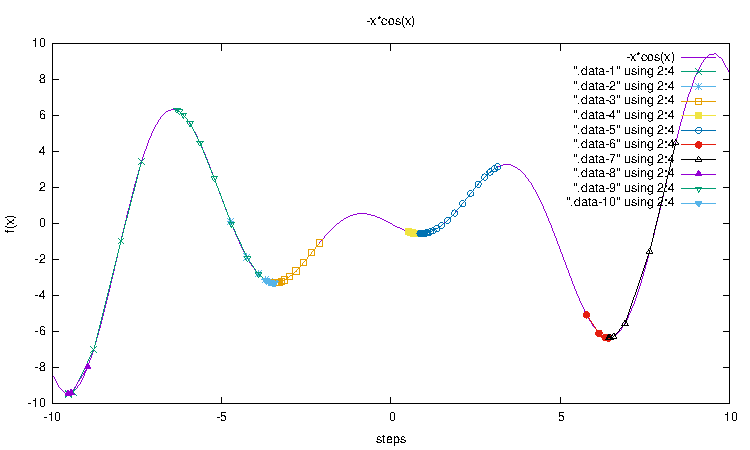
\includegraphics[width=10.0cm]{figs/level2.3/seed-1-10.pdf}
  \caption{探索初期値の変化}
	\label{trans_seed}
 \end{center}
\end{figure}

1000-10000までも,同様の結果となった.

2.異なる探索点(seed値)から複数回プログラムを実行し,局所解を比較,f(x,y)の一番小さい値を最適解として出力.
\begin{figure}[ht]
 \begin{center}
  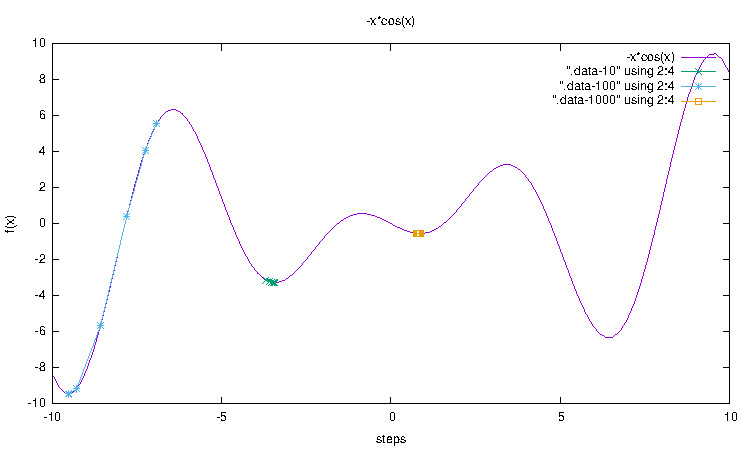
\includegraphics[width=10.0cm]{figs/level2.3/compare_seed.pdf}
  \caption{探索初期値の変化}
	\label{compare_seed}
 \end{center}
\end{figure}

\begin{breakbox}
\begin{verbatim}
% sh trans_x_vs_func_seed.sh 1000 2000 3000
FINISH 3 step 54 x and y were not updated.
FINISH 3 step 7 x and y were not updated.
FINISH 3 step 65 x and y were not updated.
seed 1000 finish f(x,y)
-0.5610963382
seed 2000 finish f(x,y)
-9.4772942595
seed 3000 finish f(x,y)
-0.5610963382
最適解は -9.477294 である
\end{verbatim}
\end{breakbox}


\subsubsection{考察}
1.まず,seed値を変更し,単体で実行したプログラムを考察していく.

初期位置が一定数値を超えなければ,定義域内での最適解に到達できず,他の局所解を最小値として出力する.

このプログラムでは,最急降下法を用いているため,切片の傾きが0となるところを目指していく.しかし,この数式だと切片の傾きが0となる最適解でない局所解を算出してしまう結果となった.

これを解決するために,2つ目の方法を使用した.
2.次に,複数のseed値を用いて比較したプログラムを考察していく.

比較にはC言語で作成したプログラムを用いた.先述したseed値を変更して同じ図に出力するシェルプログラムから最終探索値を引数として取り,その値を比較して出力した.このプログラムでは,3つの異なるseed値を使用する事によって,異なる初期位置から探索をする事ができる.

それぞれの初期位置からそれぞれの局所解を探し出す事で,解の質は大きく向上したと考える.\\

また,学習係数alphaの値を変更して探索を行うと,極端に探索回数が少なくなったが,稀に極端に探索回数が大きくなるという事が発生した.今回試した中でのalphaの最適値は0.5と判断した.
